%%%%%%%%%%%%%%%%%%%%%%%%%%%%%%%%%%%%%%%%%
% Beamer Presentation
% LaTeX Template
% Version 1.0 (10/11/12)
%
% This template has been downloaded from:
% http://www.LaTeXTemplates.com
%
% License:
% CC BY-NC-SA 3.0 (http://creativecommons.org/licenses/by-nc-sa/3.0/)
%
%%%%%%%%%%%%%%%%%%%%%%%%%%%%%%%%%%%%%%%%%

%----------------------------------------------------------------------------------------
%	PACKAGES AND THEMES
%----------------------------------------------------------------------------------------

\documentclass{beamer}

\mode<presentation> {

% The Beamer class comes with a number of default slide themes
% which change the colors and layouts of slides. Below this is a list
% of all the themes, uncomment each in turn to see what they look like.

%\usetheme{default}
%\usetheme{AnnArbor}
%\usetheme{Antibes}
%\usetheme{Bergen}
%\usetheme{Berkeley}
%\usetheme{Berlin}
%\usetheme{Boadilla}
%\usetheme{CambridgeUS}
%\usetheme{Copenhagen}
%\usetheme{Darmstadt}
%\usetheme{Dresden}
%\usetheme{Frankfurt}
\usetheme{Goettingen}	% vpravo
%\usetheme{Hannover}
%\usetheme{Ilmenau}
%\usetheme{JuanLesPins}
%\usetheme{Luebeck}
%\usetheme{Madrid}
%\usetheme{Malmoe}			
%\usetheme{Marburg}
%\usetheme{Montpellier}
%\usetheme{PaloAlto}
%\usetheme{Pittsburgh}
%\usetheme{Rochester}
%\usetheme{Singapore}			
%\usetheme{Szeged}
%\usetheme{Warsaw}

% As well as themes, the Beamer class has a number of color themes
% for any slide theme. Uncomment each of these in turn to see how it
% changes the colors of your current slide theme.

%\usecolortheme{albatross}
%\usecolortheme{beaver}
%\usecolortheme{beetle}
%\usecolortheme{crane}
%\usecolortheme{dolphin}
%\usecolortheme{dove}
%\usecolortheme{fly}
%\usecolortheme{lily}			
%\usecolortheme{orchid}
%\usecolortheme{rose}
%\usecolortheme{seagull}
%\usecolortheme{seahorse}
%\usecolortheme{whale}
%\usecolortheme{wolverine}

%\setbeamertemplate{footline} % To remove the footer line in all slides uncomment this line
%\setbeamertemplate{footline}[page number] % To replace the footer line in all slides with a simple slide count uncomment this line

%\setbeamertemplate{navigation symbols}{} % To remove the navigation symbols from the bottom of all slides uncomment this line
}

\usepackage[utf8]{inputenc}	% kódování textu
\usepackage[czech]{babel}		% zavedení češtiny
\usepackage{amsmath,amsfonts,amssymb}	% matematika
\usepackage{graphicx} % Allows including images
\usepackage{booktabs} % Allows the use of \toprule, \midrule and \bottomrule in tables
\usepackage{multirow}	% slouceni radek v tabulce
\usepackage{multicol}	% slouceni sloupcu v tabulce
\usepackage{longtable}	% rozdeleni tabulky pres vice stran
\usepackage{enumerate}	% seznamy
\usepackage{float}
\usepackage{lscape}		% stranka na sirku
\usepackage{fancyhdr}
\usepackage{url}
\usepackage{array}
\usepackage{subfigure}
\usepackage{dirtree}
\usepackage{setspace}
\usepackage{color}
\usepackage{listings}
\usepackage{multimedia}
\usepackage{tikz}
\usepackage{fancyvrb}


%------------------------------------------------------------------
%	TITLE PAGE
%------------------------------------------------------------------

\title[]{Mask R-CNN v prostředí GRASS GIS} % The short title appears at the bottom of every slide, the full title is only on the title page

\author{Ondřej Pešek} % Your name
\institute[ČVUT] % Your institution as it will appear on the bottom of every slide, may be shorthand to save space
{
České vysoké učení technické v Praze \\ % Your institution for the title page
%\medskip
Fakulta stavební \\
%\medskip
Obor Geomatika
}
\date{20. června 2018} % Date, can be changed to a custom date
\titlegraphic{
\includegraphics[width=1.5cm]{pictures/logo2.pdf}}

\begin{document}

\begin{frame}
\titlepage % Print the title page as the first slide
\end{frame}

\begin{frame}
\frametitle{Obsah} % Table of contents slide, comment this block out to remove it
\tableofcontents % Throughout your presentation, if you choose to use \section{} and \subsection{} commands, these will automatically be printed on this slide as an overview of your presentation
\end{frame}

%------------------------------------------------------------------
%	PRESENTATION SLIDES
%------------------------------------------------------------------

%------------------------------------------------------------------
\section{Motivace} % Sections can be created in order to organize your presentation into discrete blocks, all sections and subsections are automatically printed in the table of contents as an overview of the talk
%------------------------------------------------------------------

\begin{frame}

\frametitle{Motivace}

Situace
\begin{itemize}
	\item posilování satelitní sítě
	\item posilování leteckého snímkování
	\item vektorizace skenovaných map
	\visible<2->{\item zlepšování kvality snímků}
	\visible<3->{\item otevírání dat}
	\visible<4->{\item standardizace dat}
\end{itemize}

\end{frame}

%------------------------------------------------------------------

\begin{frame}

\frametitle{Motivace}

Běžné způsoby klasifikace
\begin{itemize}
	\item ruční klasifikace
	\visible<2->{\item řízená klasifikace}
	\visible<3->{\item neřízená klasifikace}
\end{itemize}

\bigskip

GRASS GIS
\begin{itemize}
	\item ruční klasifikace
	\begin{itemize}
		\item GRASS Digitizing tool
	\end{itemize}
	\visible<2->{\item řízená klasifikace
	\begin{itemize}
		\item g.gui.iclass + i.maxlik
	\end{itemize}}
	\visible<3->{\item neřízená klasifikace
	\begin{itemize}
		\item i.cluster + i.maxlik
	\end{itemize}}
\end{itemize}

\end{frame}

%------------------------------------------------------------------

\begin{frame}

\frametitle{Motivace}

Proč neuronové sítě?
\begin{itemize}
	\item mozek je nejsilnější nástroj, který máme dispozici
	\item snažíme se dosáhnout lidsky srozumitelných výsledků
\end{itemize}

\begin{figure}[ht]
	\includegraphics<1>[width=0.55\textwidth]{pictures/nn1.png}
	\includegraphics<2>[width=0.65\textwidth]{pictures/nn2.png}
	\includegraphics<3>[width=0.55\textwidth]{pictures/nn3.jpg}
	\caption{Zdroj: [1]}
\end{figure}

\end{frame}

%------------------------------------------------------------------

\section{Teoretický úvod}

\subsection{Konvoluční neuronové sítě} % A subsection can be created just before a set of slides with a common theme to further break down your presentation into chunks

%------------------------------------------------------------------

\begin{frame}

\frametitle{Konvoluční neuronové sítě}

\begin{figure}[ht]
	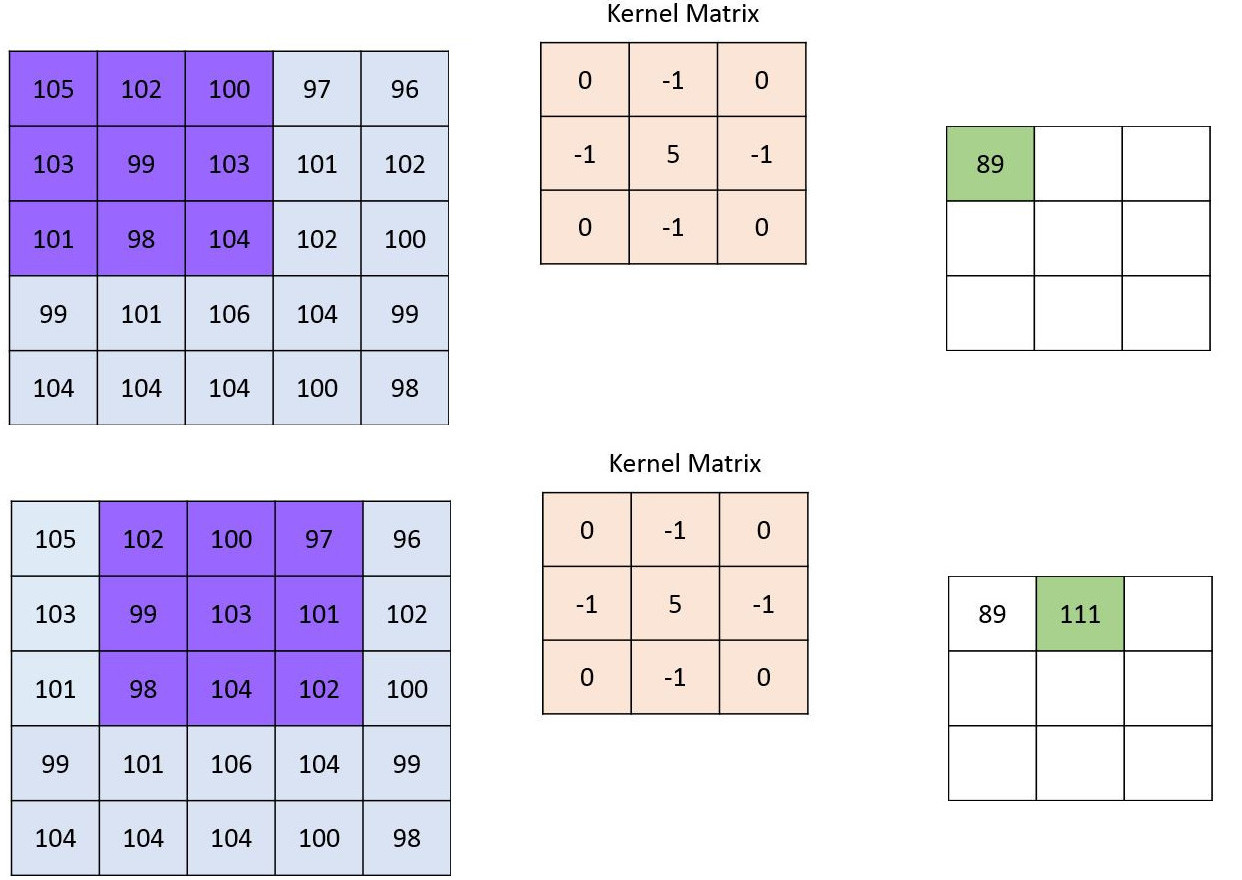
\includegraphics[width=0.6\textwidth]{pictures/conv.jpg}
\end{figure}

\visible<2->{Proč konvoluční neuronové sítě?
\begin{itemize}
	\item ResNet dosáhl v ILSVRC 2016 chybovosti 3.6 \%
	\item<3> člověk 8 \%
\end{itemize}

Zdroj: [2]}

\end{frame}

%------------------------------------------------------------------

\subsection{Mask R-CNN}

\begin{frame}

\frametitle{Mask R-CNN}

Instanční segmentace

\begin{figure}[ht]
	\includegraphics<1>[width=0.9\textwidth]{pictures/segmentations.png}
	\includegraphics<2>[width=0.65\textwidth]{pictures/instance-segmentation.png}
	\caption{Zdroj: [3]}
\end{figure}

\end{frame}

%------------------------------------------------------------------

\begin{frame}

\frametitle{Mask R-CNN}

Dvě části:
\begin{itemize}
	\item páteřní
	\item hlavová
\end{itemize}

\begin{figure}[ht]
	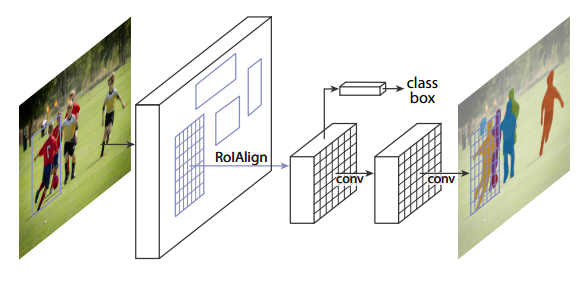
\includegraphics[width=0.8\textwidth]{pictures/maskrcnn.png}
	\caption{Zdroj: [4]}
\end{figure}

\end{frame}

%------------------------------------------------------------------

\begin{frame}

\frametitle{Mask R-CNN}

Páteřní architektura:
\begin{itemize}
	\item ResNet
	\item<2-> RPN
\end{itemize}

\begin{figure}[ht]
	\includegraphics<1>[width=0.5\textwidth]{pictures/bottleneck-block.jpg}
	\includegraphics<2>[width=0.5\textwidth]{pictures/fasterrcnn.png}
	\includegraphics<3>[width=0.5\textwidth]{pictures/fasterrcnn-anchors.png}
	\caption{Zdroj: [4]}
\end{figure}

\end{frame}

%------------------------------------------------------------------

\begin{frame}

\frametitle{Mask R-CNN}

Hlavová architektura:
\begin{itemize}
	\item softmax $\rightarrow$ třída
	\item<2-> regrese $\rightarrow$ ohraničující obdélník
	\item<3-> plně spojené vrstvy $\rightarrow$ maska
\end{itemize}

\begin{figure}[ht]
	\includegraphics<1-2>[width=\textwidth]{pictures/fastrcnn.png}
	\includegraphics<3>[width=\textwidth]{pictures/maskrcnn-head.png}
	\caption{Zdroj: [5]}
\end{figure}

\end{frame}

%------------------------------------------------------------------

\section{Implementace}

%------------------------------------------------------------------

\subsection{Použití}

\begin{frame}

\frametitle{Použití}

Postup práce:
\begin{itemize}
	\item i.ann.maskrcnn.train
	\item i.ann.maskrcnn.detect
\end{itemize}

\end{frame}

%------------------------------------------------------------------

\subsection{i.ann.maskrcnn.train}

\begin{frame}

\frametitle{i.ann.maskrcnn.train}

Postup práce modulu
\begin{itemize}
	\item<1-> konfigurace modelu
	\item<2-> naplnění předtrénovanými váhami
	\item<3-> přečtení datasetu
	\item<4-> učení
	\item<5-> uložení modelu
\end{itemize}

\begin{figure}[ht]
	\includegraphics<1>[width=.7\textwidth]{pictures/gui-train-conf.png}
	\includegraphics<2>[width=.7\textwidth]{pictures/gui-train-weights.png}
	\includegraphics<3>[width=.7\textwidth]{pictures/gui-train-dataset.png}
	\includegraphics<4>[width=.7\textwidth]{pictures/gui-train-train.png}
	\includegraphics<5>[width=.7\textwidth]{pictures/gui-train-save.png}
\end{figure}

\end{frame}

%------------------------------------------------------------------

\subsection{i.ann.maskrcnn.detect}

\begin{frame}

\frametitle{i.ann.maskrcnn.detect}

Postup práce modulu
\begin{itemize}
	\item<1-> naplnění natrénovanými váhami
	\item<2-> detekce pro každý obrázek
	\item<3-> vektorizace
\end{itemize}

\begin{figure}[ht]
	\includegraphics<1>[width=.7\textwidth]{pictures/gui-detect-model.png}
	\includegraphics<2>[width=.7\textwidth]{pictures/gui-detect-images.png}
	\includegraphics<3>[width=.7\textwidth]{pictures/gui-detect-vectorize.png}
\end{figure}

\end{frame}

%------------------------------------------------------------------

\subsection{Výsledky}

\begin{frame}

\frametitle{Výsledky}

\begin{figure}[ht]
	\only<1>{
	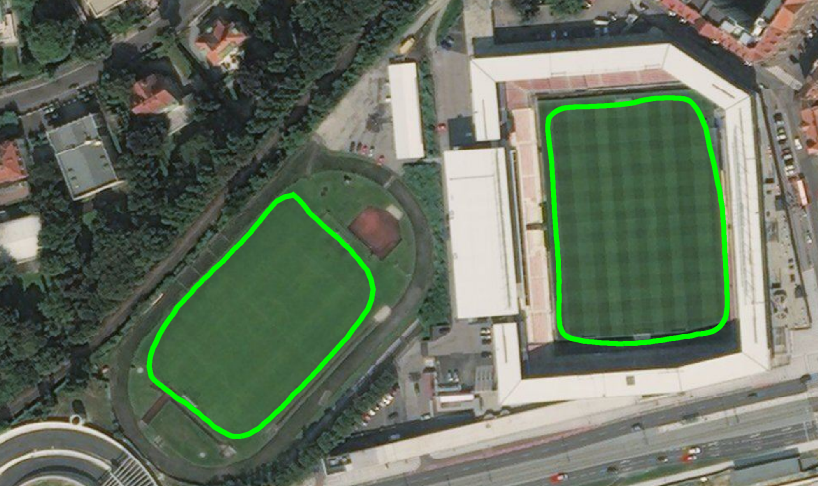
\includegraphics[width=.9\textwidth]{pictures/out1.png}
	\caption{ztrátová funkce 0.96, 54000 trénovacích obrázků}}
	\only<2>{
	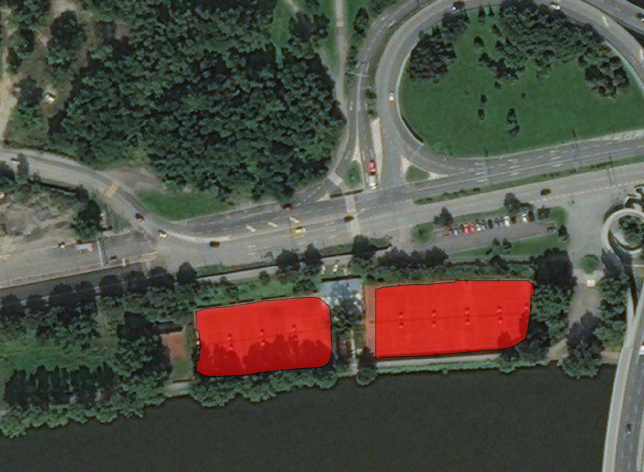
\includegraphics[width=.9\textwidth]{pictures/out2.png}
	\caption{ztrátová funkce 0.96, 54000 trénovacích obrázků}}
	\only<3>{
	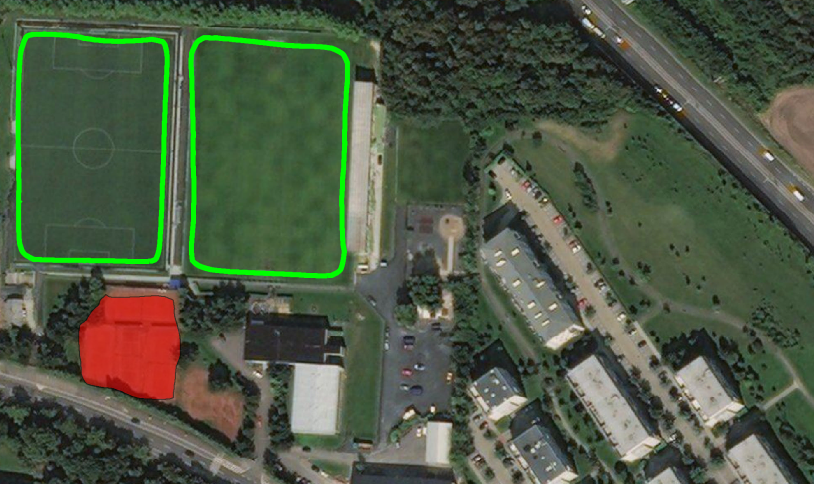
\includegraphics[width=.9\textwidth]{pictures/out3.png}
	\caption{ztrátová funkce 0.96, 54000 trénovacích obrázků}}
	\only<4>{
	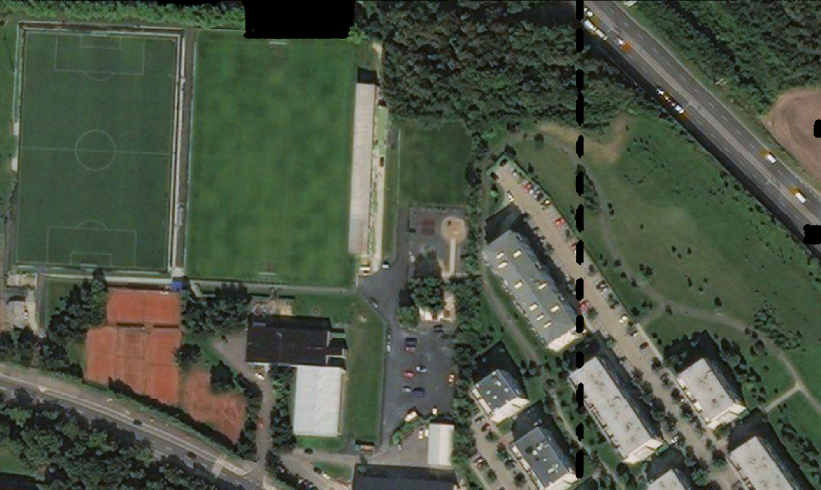
\includegraphics[width=.9\textwidth]{pictures/out_b_1.png}
	\caption{epocha 1, ztrátová funkce 35.01, 2400 trénovacích obrázků}}
	\only<5>{
	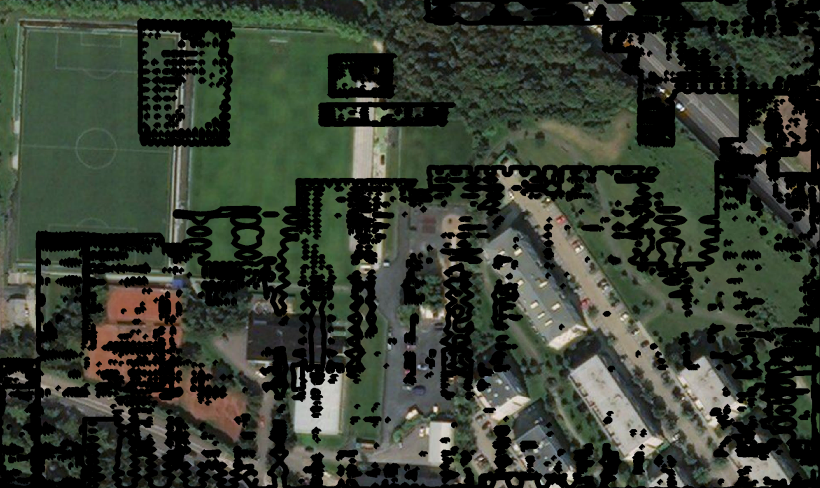
\includegraphics[width=.9\textwidth]{pictures/out_b_10.png}
	\caption{epocha 10, ztrátová funkce 5.87, 2400 trénovacích obrázků}}
	\only<6>{
	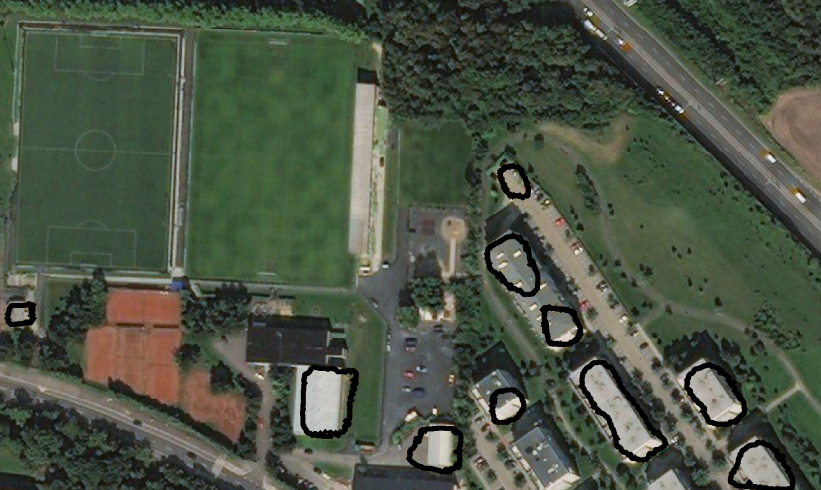
\includegraphics[width=.9\textwidth]{pictures/out_b_50.png}
	\caption{epocha 50, ztrátová funkce 1.36, 2400 trénovacích obrázků}}
	\only<7>{
	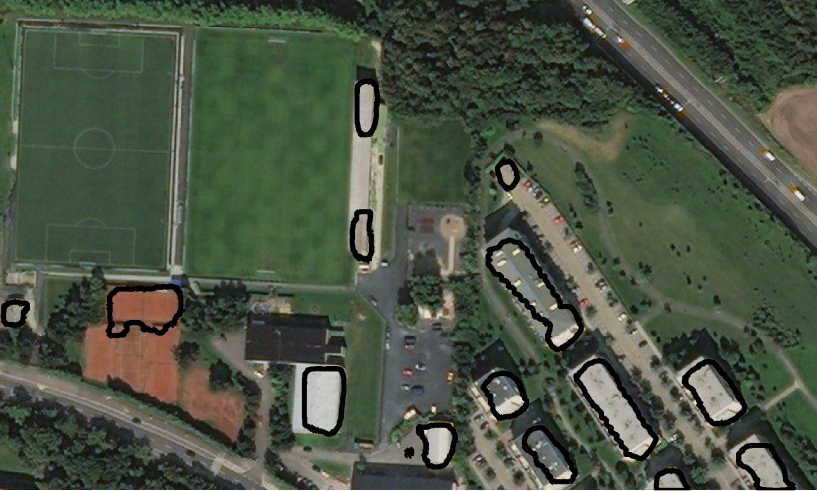
\includegraphics[width=.9\textwidth]{pictures/out_b_150.png}
	\caption{epocha 150, ztrátová funkce 0.63, 2400 trénovacích obrázků}}
	\only<8>{
	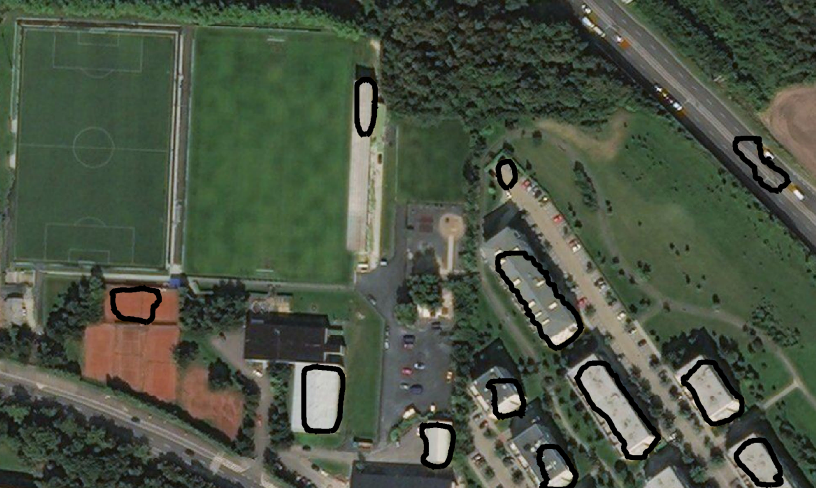
\includegraphics[width=.9\textwidth]{pictures/out_b_180.png}
	\caption{epocha 180, ztrátová funkce 0.50, 2400 trénovacích obrázků}}
\end{figure}

\end{frame}

%------------------------------------------------------------------

\section{Závěr}

\begin{frame}[fragile]

\frametitle{Závěr}

\begin{itemize}
	\item zdrojový kód
	\begin{itemize}
		\item \url{https://github.com/ctu-geoforall-lab-projects/dp-pesek-2018}
		\item \url{https://svn.osgeo.org/grass/grass-addons/grass7/imagery/i.ann.maskrcnn/}
	\end{itemize}
	\item instalace pomocí příkazu \verb|g.extension extension=i.ann.maskrcnn|
	\item další vývoj
	\begin{itemize}
		\item \url{https://github.com/ctu-geoforall-lab/i.ann.maskrcnn}
		\item multispektrální rastry
		\item učení na rastrech importovaných v prostředí GRASS
		\item další architektury
	\end{itemize}
\end{itemize}

\end{frame}

%------------------------------------------------------------------

\section{Zdroje}

\begin{frame}

\frametitle{Zdroje}

[1] https://www.analyticsvidhya.com/blog/2016/04/deep-learning-computer-vision-introduction-convolution-neural-networks/

[2] RUSSAKOVSY, Olga et al.
ImageNet Large Scale Visual Recognition
Challenge. International Journal of Computer Vision IJCV. 2015, 115, n. 3,
pp. 211–252.

[3] http://cs231n.stanford.edu/

[4] HE, Kaiming et al. Mask R-CNN. In: International Conference on Computer
Vision (ICCV). 2017.

[5] GIRSHICK, Ross. Fast R-CNN. In: International Conference on Computer
Vision (ICCV). 2015.

\end{frame}

%------------------------------------------------------------------

\begin{frame}

\Huge{\centerline{Děkuji za pozornost.}}

\end{frame}

%------------------------------------------------------------------

\section{Reakce na otázky oponenta}

\begin{frame}

\frametitle{Reakce na otázky oponenta}

Jaké jsou výhody/nevýhody užití neuronových sítí namísto klasických postupů?

\begin{center}
	\noindent\makebox[\linewidth]{\rule{0.9\textwidth}{0.4pt}}
\end{center}

\bigskip

Výhody:
\begin{itemize}
	\item<2-> přesnost
	\item<3-> minimalizovaná potřeba vytvářet ad hoc řešení
	\item<4-> obecnost
\end{itemize}

Nevýhody:
\begin{itemize}
	\item<5-> výpočetní náročnost
	\item<6-> časová náročnost
	\item<7-> potřeba rozsáhlých trénovacích dat
	\item<8-> odvážným štěstí nepřeje vždy
\end{itemize}

\end{frame}

%------------------------------------------------------------------

\begin{frame}

\frametitle{Reakce na otázky oponenta}

Implementoval jste modifikace využitého software i zpět do zdrojů?

\begin{center}
	\noindent\makebox[\linewidth]{\rule{0.9\textwidth}{0.4pt}}
\end{center}

\bigskip

Ano:
\begin{itemize}
	\item<2-> GRASS GIS
\end{itemize}

Ne:
\begin{itemize}
	\item<3-> GRASS GIS
	\item<4-> Matterport, Inc.
	\item<7-> potřeba rozsáhlých trénovacích dat
	\item<8-> odvážným štěstí nepřeje vždy
\end{itemize}

\end{frame}

%------------------------------------------------------------------

\begin{frame}

\frametitle{Reakce na otázky oponenta}

Shledáváte některé části svého kódu natolik obecnými, aby mohly být využiti i při vývoji dalších podobných nástrojů?

\begin{center}
	\noindent\makebox[\linewidth]{\rule{0.9\textwidth}{0.4pt}}
\end{center}

\bigskip

\visible<2->{Ano.}

\end{frame}

%------------------------------------------------------------------

\begin{frame}

\frametitle{Reakce na otázky oponenta}

V textu práce jste zmínil a rozebíral podezřelé chování modulů skýtajících lepší výsledky při vyšší ztrátové funkci. Můžete tento případ ještě rozvést?

\begin{center}
	\noindent\makebox[\linewidth]{\rule{0.9\textwidth}{0.4pt}}
\end{center}

\bigskip

Možné příčiny:
\begin{itemize}
	\item<2-> přeoptimalizace
	\item<3-> lokální odchylka
	\item<4-> nedostatečná data
\end{itemize}

\begin{figure}
	\centering
	\begin{minipage}{.45\textwidth}
		\centering
		\begin{figure}[ht]
	  		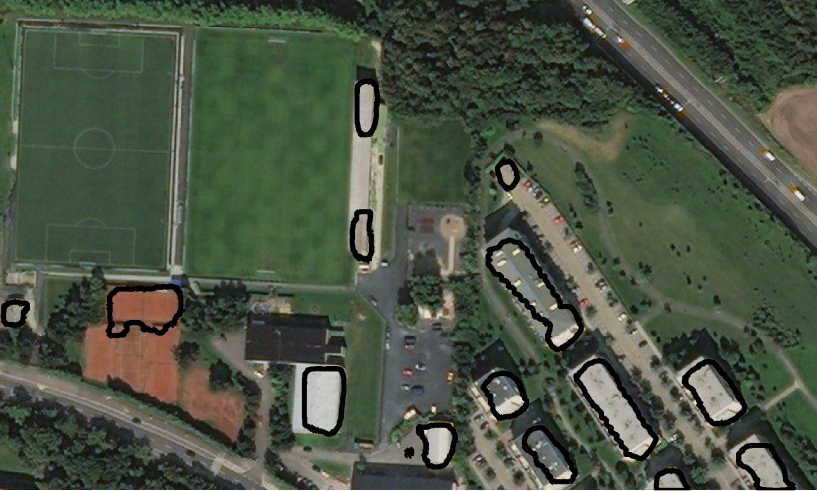
\includegraphics[width=4.5cm]{pictures/out_b_150.png}
		\end{figure}
    \end{minipage}%
    \begin{minipage}{.6\textwidth}
		\centering
		\begin{figure}[ht]
			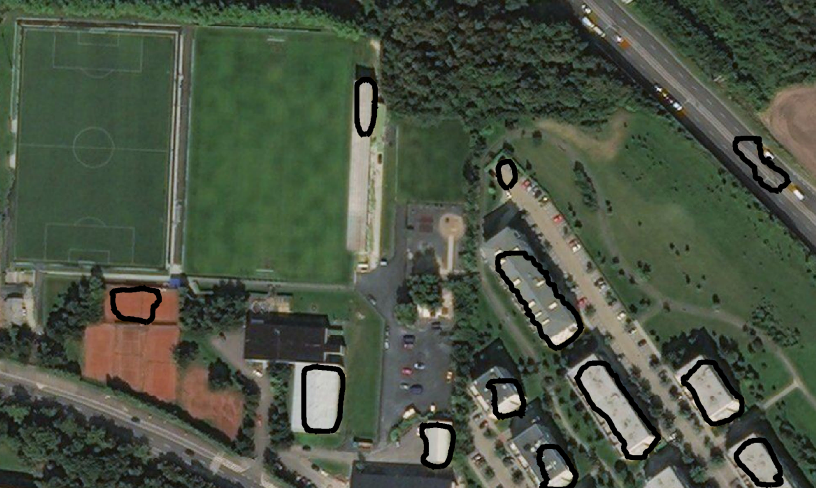
\includegraphics[width=4.5cm]{pictures/out_b_180.png}
		\end{figure}
	\end{minipage}
\end{figure}

\end{frame}

%==================================================================
\end{document} 

